\section{Case Study}
\label{CaseStudy}
In this section, a case study is introduced to verify the feasibility and effectiveness of the approaches above. We construct a prototype system, EVER, an intelligent charging pile sharing platform, to illustrate a typical application of our framework. 

As a kind of WoT equipment, intelligent charging pile is connected to the Internet through WIFI or GPRS, offering RESTful services as operation interfaces. In China, charging pile sharing is an emerging area. The owner can make his private charging pile open to the public, and the public can charge their car by paying a certain fee to the owner. The sharing platform brings a win-win pattern, as the lack of public charging pile can be alleviated and the owner can cover the cost of building the charging pile through the income. 

A brief process of charging through the sharing platform has following steps:
\begin{itemize}
\setlength{\itemsep}{1pt}
\setlength{\parskip}{0pt}
\setlength{\parsep}{0pt}
\item When a driver need to charge his car, he can open the App on his smart phone to fetch all the candidate charging piles nearby. 
\item Then, he can choose a pile and check the detail information of it, including suitable car type, available time, charging fee and etc. 
\item If the pile is suitable, he can make a reservation in his App. 
\item After arriving the charging pile, he can scan the QR code on the charging pile to start charging. 
\item When the charging is over, he can stop the charging in his App and get the bill to pay. 
\end{itemize}

During the charging process, several device services are used to perform business functionalities such as making reservation and generating bill. However, as there are hundreds of different charging pile models in the market, how to adapt the business process to all those models is a great challenge. 

Based on our framework, we designed and implemented a sharing platform, EVER, which has a strong adaptability for the cross-devices process reuse. 

\subsection{Application of the framework}
Reviewing the business process of charging, we found that most activities in the process are related to one or more device services. Therefore, with the help of our Eclipse modeling plugin, we have described those activities in the activity description model. An example of those descriptions is introduced in Fig.~\ref{fig_activitydescriptionmodeldemo}. 

\begin{figure}[!t]
\centering
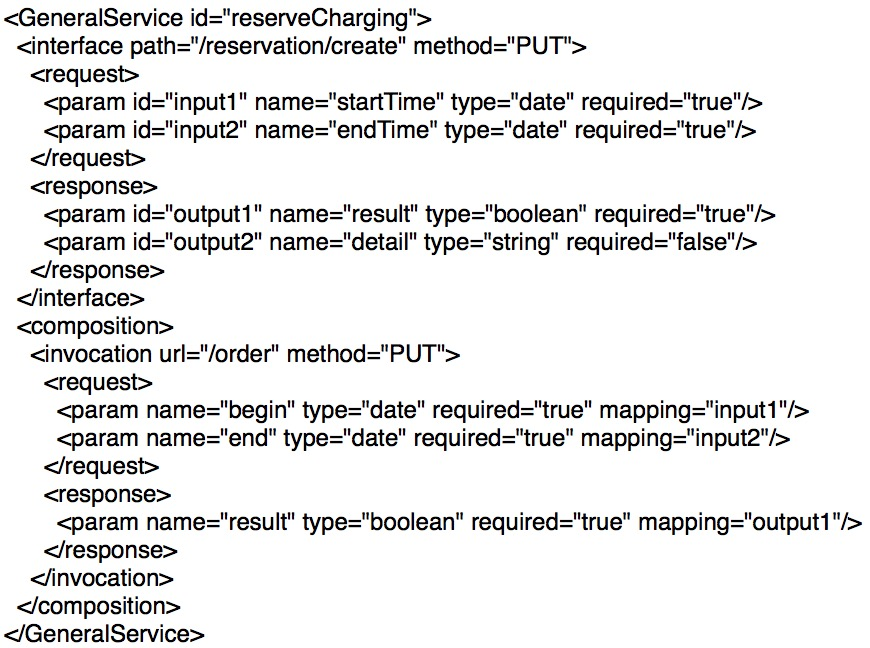
\includegraphics[width=1.0\linewidth]{./graph/generalservicedemo}
% where an .eps filename suffix will be assumed under latex, 
% and a .pdf suffix will be assumed for pdflatex; or what has been declared
%via \DeclareGraphicsExtensions.
\caption{An example of general service model.}
\label{fig_generalservicedemo}
\end{figure}

When a pile owner want to register and share his pile on our platform, the WADL documents of device services should be uploaded. With those descriptions, our matching algorithm is exectued to generate the general service models. Fig.~\ref{fig_generalservicedemo} serves as an example of a general service model.
In the model, the $invocation$ node presents a device service interface for the functionality of reserving charging, which is bound to the general "/reservation/create" service. 

Based on the sample model, source code of the general service can be generated, which is shown in Fig.~\ref{fig_generalservicedemo}. After the general services are deployed on the pile, the pile is now available to the public. 

When a user calls a general service, the general service will help the user to invoke real services on the device. Consequently, our general service offers a device-independent interface to users, which hide all the device services from the user. 

\subsection{Implementation of the system}
EVER is consist of four parts: center server, web site, App and intelligent charging pile. The pile provides RESTful services for the device resources. The center server is in charge of the other APIs of the system. The web site offers user interface for the management of the intelligent charging piles, such as updating the pile state or checking the usage record. Fig.~\ref{fig_prototype1} presents the web page for sharing a new charging pile. The App provides the main charging business. Users can make the reservation, control the charging and pay for bill on the App. The reservation and charging pages of the App is shown in Fig.~\ref{fig_app}. 

\begin{figure}[!t]
\centering
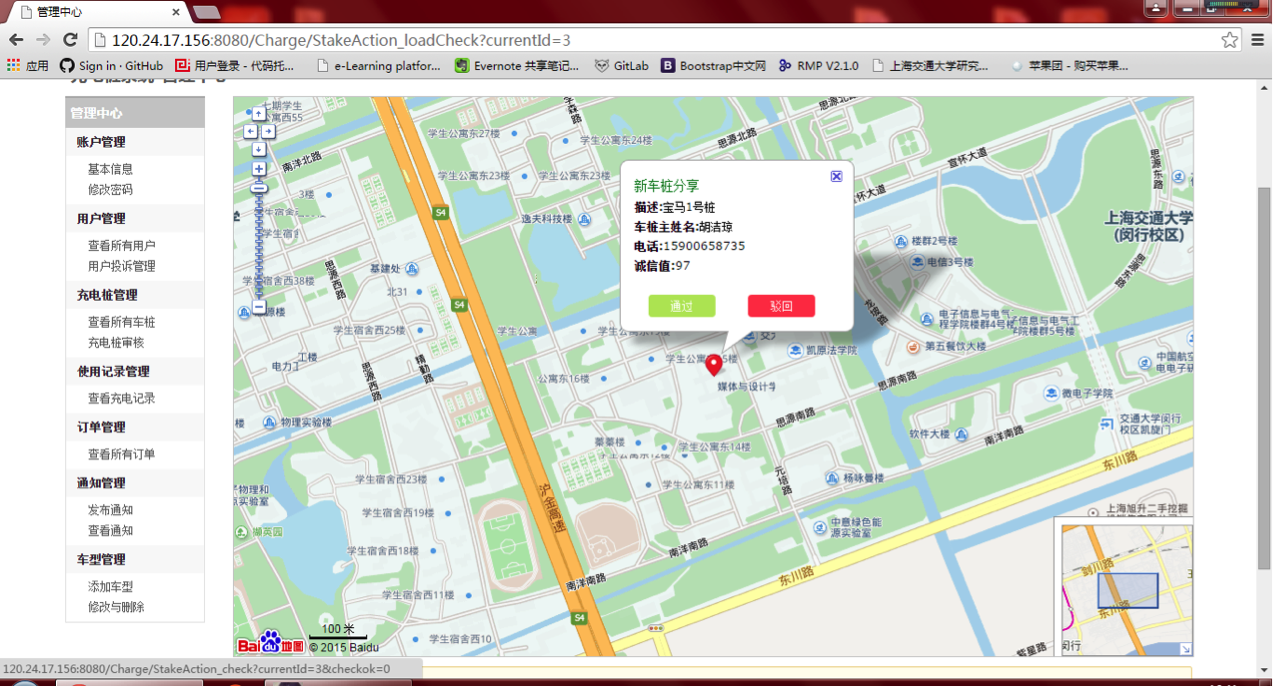
\includegraphics[width=1.0\linewidth]{./graph/prototype1}
% where an .eps filename suffix will be assumed under latex, 
% and a .pdf suffix will be assumed for pdflatex; or what has been declared
%via \DeclareGraphicsExtensions.
\caption{A screenshot of the prototype system.}
\label{fig_prototype1}
\end{figure}

\begin{figure}[!t]
\centering
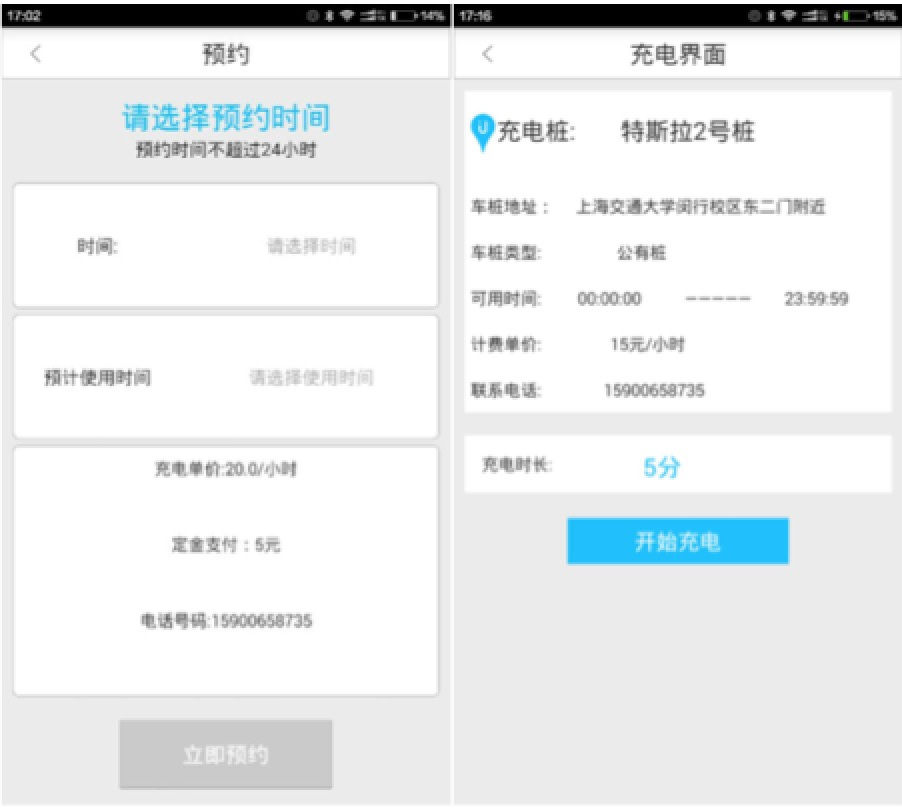
\includegraphics[width=1.0\linewidth]{./graph/app}
% where an .eps filename suffix will be assumed under latex, 
% and a .pdf suffix will be assumed for pdflatex; or what has been declared
%via \DeclareGraphicsExtensions.
\caption{Screenshots of the App.}
\label{fig_app}
\end{figure}

